\documentclass{beamer}

\usetheme{Boadilla}
\usepackage{colortbl}
\usepackage{multimedia}
\usepackage{comment}
\usepackage{graphics}


\definecolor{pink}{rgb}{0.8,0.6,0.6}
\definecolor{blue}{rgb}{0.2,0.2,0.8}
\setbeamertemplate{frametitle}[default][center]
\setbeamertemplate{navigation symbols}{}
\setbeamercolor{item}{fg=red}
\setbeamertemplate{items}[square]

%% Macro
\def\x{\mathbf{x}}
\def\R{\mathbb{R}}
\def\n{\mathbf{n}}
%%

 \title{A simple approach to mesh deformation}
\author{Shingo Ito}
\institute{s1200045}
\date{\today}

\begin{document}
\titlepage
%% page 1 : title


%page2
\section{Introduction}


\begin{frame}
	\frametitle{Introduction}
	\Large
	\begin{itemize}
   \item Present a simple approach for mesh deformation.
		%\begin{block}{What is Metamorphosis of shapes?}
		\item Sampling of the deformed mesh obtained from applying a surface reconstruction algorithm to the deformed point cloud. \\
		\end{itemize}
	%\end{block}
\end{frame}
%page3
\section{Related works}
\begin{frame}
\frametitle{Related works}
\Large
\begin{itemize}
\item Surface deformation is an important research topic in shape and geometric modeling.
\item The main technique consists in computing an approximation of the distance to the zero level-set and deforming this distance field.
\end{itemize}
\end{frame}

%page4
\section{Algorithm overview}
\begin{frame}
	\frametitle{Algorithm overview}
	\Large
Surface deformation work by moving the triangle mesh vertices according to some specified vector field corresponding to the deformation.
		\begin{itemize}
			\item Sample from the surface
			\item Apply the deformation field to the samples
			\item Apply a surface reconstruction algorithm to the samples
			\end{itemize}
\end{frame}


%page5
\section{Algorithm and implimentation details}
\Large

\begin{frame}
\frametitle{Surface sampling}
Uniform sampling from a triangle\\
\begin{itemize}
\item Function Sample($p_1$, $p_2$, $p_3$, $\xi_1$, $\xi_2$)\\

\  $p_1$, $p_2$ and $p_3$ are the triangle vertices, $\xi_1$ and $\xi_2$ are samples from a uniform distribution\\

\  Compute the barycentric coordinates: $u = 1-\sqrt{\xi_1}$ and $v = \xi_2 \sqrt{\xi_1}$\\

\  Compute the sample: $P = u * p_1 + v * p_2 + (1 - u - v) * p_3$\\
\   return $P$\\
end function
\end{itemize}
\end{frame}


\begin{frame}
	\frametitle{Points deformation}

		Given a selected vertex from the input surface. \\
		Apply a truncated Gaussian centered on this selected vertex \\
\[f(x)=
\begin{cases}

 \frac{1}{\sqrt{2\pi \sigma}} \exp \left(- \frac{(\x- \x_S)^{2}}{2 \sigma^{2}}\right) & \text{if } \|\ x-\x_S\| < \epsilon \\
0 & \text{otherwise}
\end{cases}
\]
\end{frame}

\begin{frame}
	\frametitle{Surface reconstruction}
	\Large
	Implemented and experimented with three surface reconstruction algorithms.\\
	All approaches are implicit surface based surface reconstruction algorithms\\
\[f: \R^3 \rightarrow \R\]
\end{frame}


\begin{frame}
	\frametitle{Hermite Radial Basis Functions}
	\Large
Given a set of points $P = {\x_i}$ with normal vector at each point $N = {\n_i}$, 
the output of the method is a function: $f : \R^3 \to \R$ defined as follows:
\[
f(\x)=\sum_{i=1}^n(\alpha_i\phi(\|\x-\x_i\|)-\beta_i\nabla\phi(\|\x-\x_i\|))
\]

\end{frame}


\begin{frame}
\frametitle{Hermite Radial Basis Functions}
\Large
The conditions used to determine the coefficients are: \[f(\x_i) = 0, \x_i \in \R^3\]
for interpolating points on the surface. And: \[\nabla f(\x_i)=\n_i, \x_i \in \R^3, \n_i \in \R^3\]
for interpolating the normals on the surface.

\end{frame}


\begin{frame}
\frametitle{Hermite Radial Basis Functions}
\Large
\[f(\x_i)=\sum_{j=1}^n(\alpha_j\phi(\|\x_i-\x_j\|)-\beta_j\nabla\phi(\|\x_i-\x_j\|))=0\]
\[\nabla f(\x_i)=\sum_{j=1}^n(\alpha_j\nabla\phi(\|\x_i-\x_j\|)-H\phi(\|\x_i-\x_j\|)\beta_j)=\n_i\]
where $H$ is the Hessian matrix of $\phi$.
\end{frame}


\begin{frame}
	\frametitle{Hermite Radial Basis Functions}
	\Large
	\begin{align} \label{hrbf1}
 & \sum_{j=1}^n
\begin{bmatrix}
\phi(\|\x_i-\x_j\|) & -\nabla\phi(\|\x_i-\x_j\|)^T\\ \nabla\phi(\|\x_i-\x_j\|) & -H\phi(\|\x_i-\x_j\|)
\end{bmatrix}
\begin{bmatrix}
\alpha_j\\\beta_j
\end{bmatrix} \nonumber
\\
 & + \sum_{l=1}^m\lambda_l
\begin{bmatrix}
p_l(\x_i)\\\nabla p_l(\x_i)
\end{bmatrix}
=
\begin{bmatrix}
0 \\ \n_i
\end{bmatrix}
\end{align}
%\]
With the additional condition:
\begin{equation} \label{hrbfcond}
\sum_{j=1}^n[p_k(x_j)\nabla p_k(x_j)^T]\begin{bmatrix}\alpha_j\\\beta_j\end{bmatrix}=0
\end{equation}

\end{frame}


\begin{frame}
	\frametitle{Hermite Radial Basis Functions}
	\Large
\[\nabla\phi(\|x\|) = 3x\|x\|\]
\[ H \phi (\|x\|)= \left\{ \begin{array}{ll} 3/\|x\|(\|x\|^2I_{3\times3}) + xx^T, & \|x\| \neq 0\\ 
0_{3\times3}, &\|x\| = 0 \end{array}\right.\]
\end{frame}


\begin{frame}
\frametitle{Closed form solution for compactly supported functions}
\Large
\begin{equation} \label{hrbfclosed}
f(x)=-\sum_{j=1}^n<\frac{\rho^2_j}{20+\eta\rho^2_j} \n_j, \nabla\phi_{\rho_j}(\|\x-\x_j\|)>
\end{equation}
where $\rho_j$ is the radius of support of the basis function associated to the center $j$, 
and $\phi$ is the compactly supported basis function. 
\[
\phi_{\rho}(r)=\phi(r/\rho)
\]
where:
\[
\phi (t)= \left\{ \begin{array}{ll} (1-t)^{4}(4t+1), & t \in [0,1]\\ 
0, & \text{otherwise} \end{array}\right.
\]

\end{frame}

\begin{frame}
	\frametitle{Poisson surface reconstruction}
\[
f_S (\x)= \left\{ \begin{array}{ll} 1 & \x \in S\\ 
0 & otherwise \end{array}\right.
\]\\
The indicator function
$f$ is obtained by solving the Poisson equation
\[
\Delta f=div(\n)
\]
where $\n$ is an extrapolation of the given normal vector field.
\end{frame}


\begin{frame}
\frametitle{Marching Cubes}
\Large
Algorithm for rendering isosurfaces from volumetric data. \\
\begin{itemize}
\item Bounding box for the object to be meshed and subdivide it regularly into smaller cells. 
\item the function f is sampled at the eight corners of each cell.
\item If one or more values is less than the user-specified iso-value, and one or more have values is greater than this isovalue, the cell must intersect the isosurface.
\end{itemize}
\end{frame}


\begin{frame}
\frametitle{Marching Cubes}
\Large
\begin{itemize}
\item Determining the edges in the cell that are intersected by the isosurface.
\item connecting the patches from all cells, we get a linear approximation of the isosurface.
\end{itemize}
\end{frame}

\begin {frame}
\frametitle{Delaunay based implicit surface meshing}
\Large
\begin{itemize}
\item Marching Cubes based algorithm do not look like the most effective approach.\\
\item Compute a Delaunay tetrahedralization of the deformed point-cloud.\\
\item Peel off outside tetrahedra using the fitted function\\
\end{itemize}
\end{frame}


\section{Experiments and result}

\begin{frame}
\frametitle{The environment used for prototype and in the experiments}
\Large
The development and all experiments were run on a regular note PC. \\
\begin{table}
\begin{center}
\begin{tabular}{|p{3cm}|p{7cm}|} 
\hline
CPU & Intel Corei5 1.4GHz \\ 
\hline
GPU & Intel HD Graphics5000 \\ 
\hline
Memory & 4.0GB RAM \\ 
\hline
OS & OS X Yosemite ver- sion 10.10.5 \\  
\hline
Programming Language & C++ \\
\hline 
Libraries & CGAL4.7,OpenGL,Eigen \\ 
\hline
\end{tabular}
\end{center}
\end{table}

\end{frame}


\begin{frame}
	\frametitle{Deformation of a sphere}
 Start from a sphere repre-sented by a triangle mesh, made of 174 vertices and 344 triangles. \\
 \begin{figure}
 \centering
 \hbox{
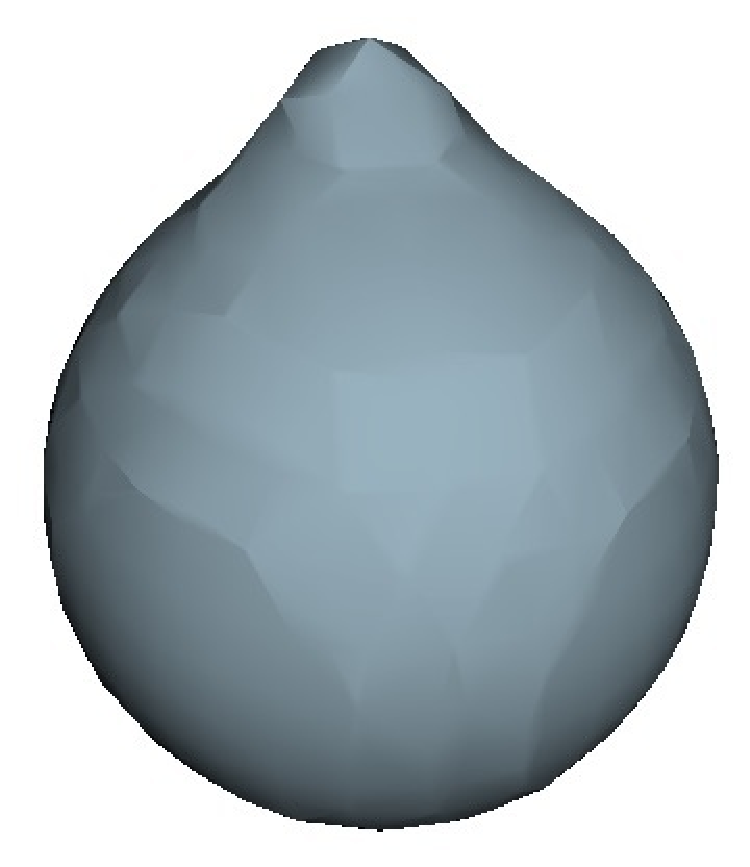
\includegraphics[width=0.30\columnwidth]{deformedspherehrbf.eps}
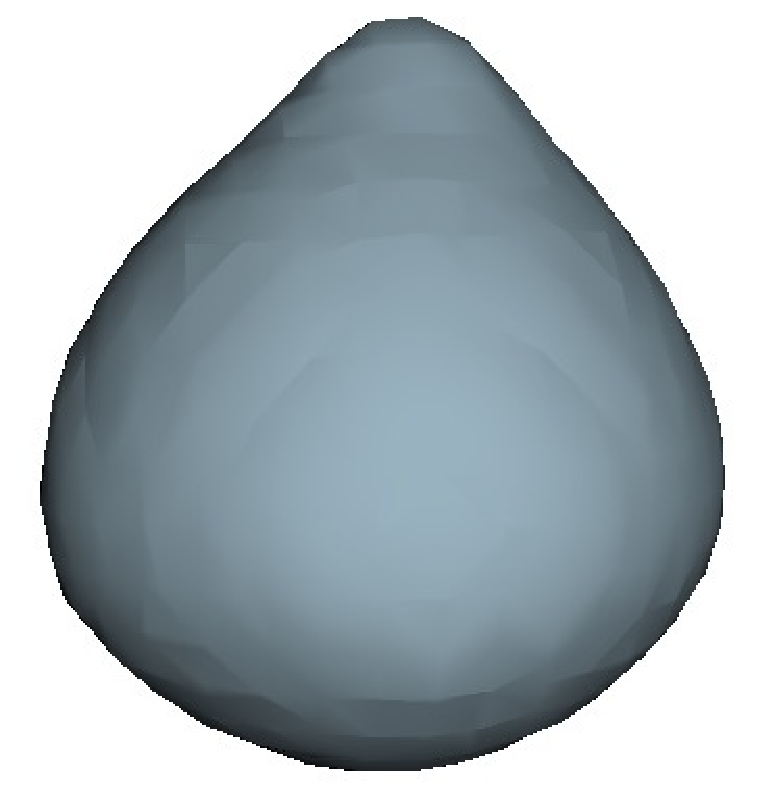
\includegraphics[width=0.30\columnwidth]{deformedspherehrbfclosed3.eps}
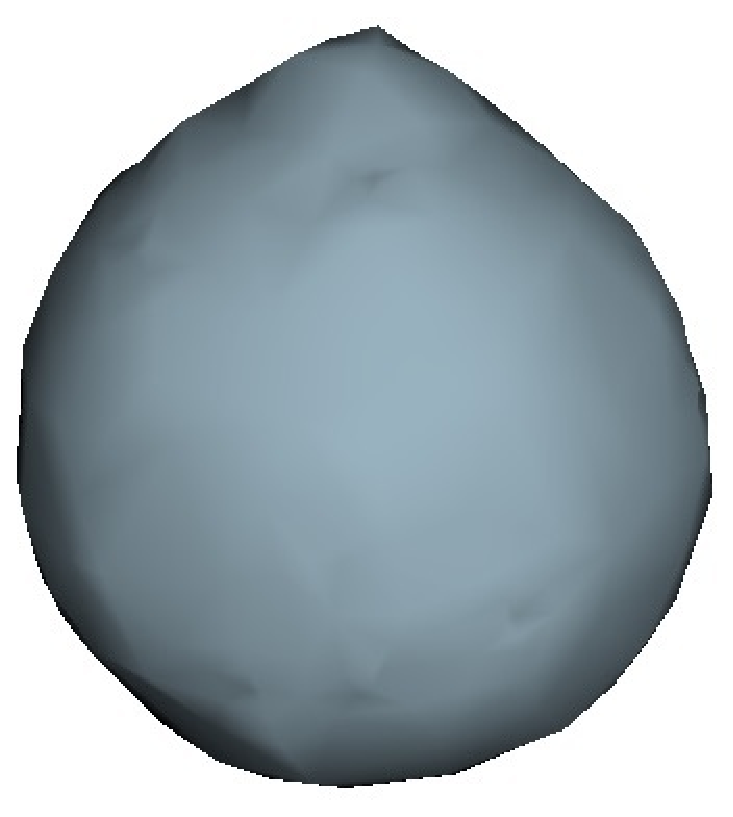
\includegraphics[width=0.30\columnwidth]{deformedspherepoisson.eps}
}
\caption{Deformed sphere using (from left to right): the HRBF approach, 
the closed form solution to the HRBF approach and the Poisson surface
reconstruction approach}
\end{figure} 
\end{frame}

\begin{frame}
\frametitle{Example of sculpture}
\Large
\begin{figure}
  \centering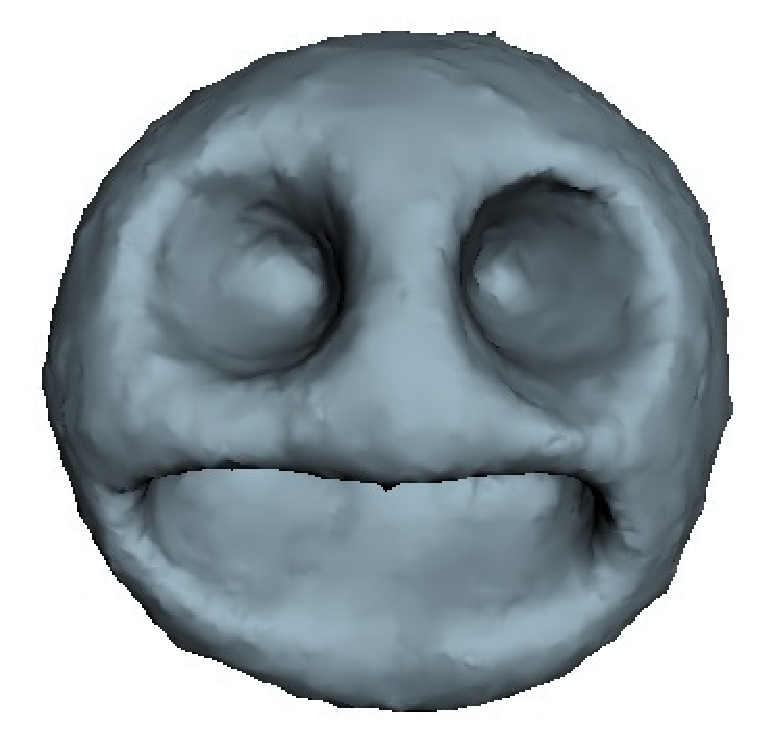
\includegraphics[width=0.3\columnwidth]{simplefacepoisson2.eps}
  \caption{Example to model a simple character face} \label{fig:face}
\end{figure}
\begin{itemize}
\item The eyes and the mouth were carved by changing the sign of the field used for the deformation.
\item Changing the width of the Gaussian function used for the deformation could allow to add or carve smaller details.
\end{itemize}
\end{frame}

\begin{frame}
\frametitle{Deformation of a more complex surface}
\begin{figure}
  \centering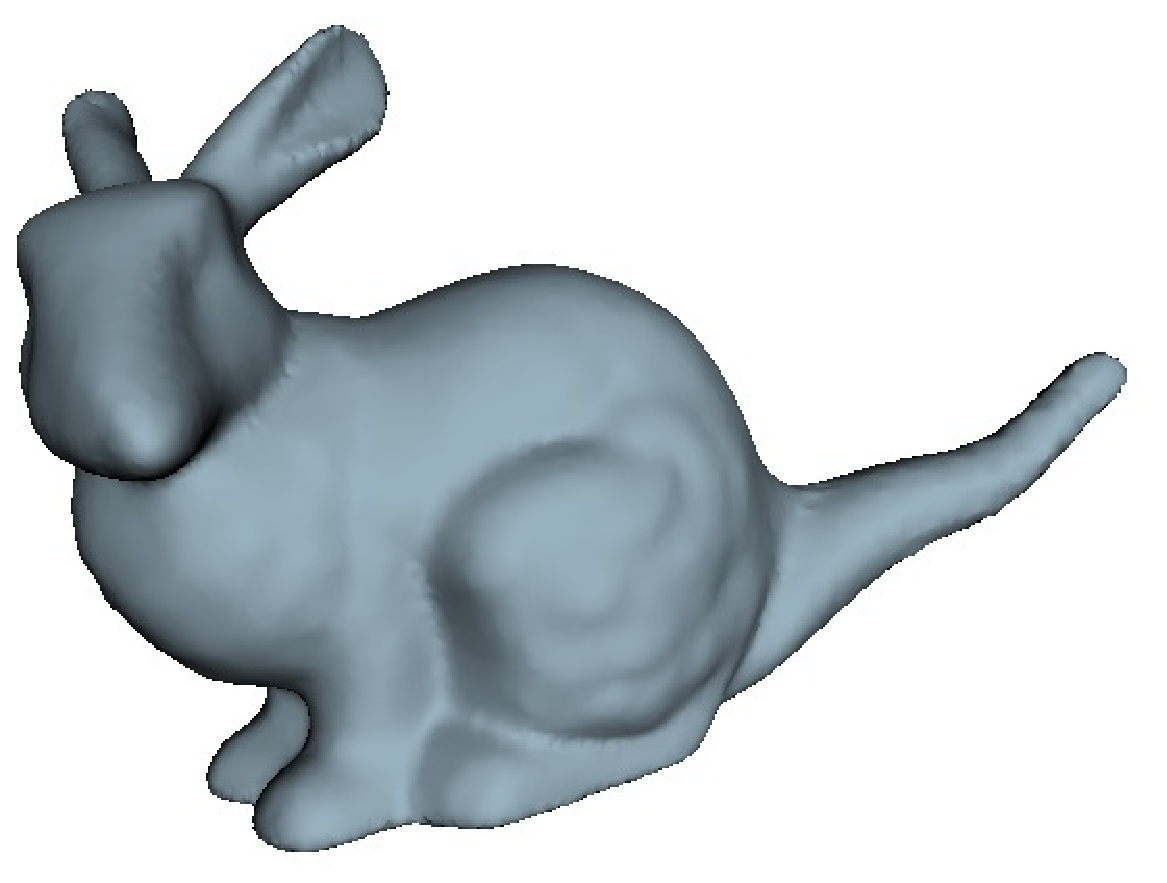
\includegraphics[width=0.4\columnwidth]{deformedbunnypoisson.eps}
  \caption{Deformed bunny object with stretched tail and nose} \label{fig:bunnyPoisson}
\end{figure}

\Large
\begin{itemize}
\item The input mesh for this object contains 14072 vertices and 28042 triangles.
\item  Both the tail and the nose are stretched.
\end{itemize}


\end{frame}

\begin{frame}
\frametitle{Conclusion}
\begin{itemize}
\item Proposed a simple algorithm for mesh deformation.
\item Reconstruction from the point-cloud is made by fitting an implicit surface to the point-cloud and meshing it.
\item Future works : Implementing parts of the algorithm on the graphics card (GPU).
\end{itemize}
\end{frame}
\begin{frame}
\frametitle{ {\color{blue}.}}
\centering
\Large
Thank you.

\end{frame}


\end{document}